\subsubsection*{Regularização}

Quando se modela uma arquitetura de redes neurais, pode-se chegar a três casos, sendo eles: subajuste (\textit{underfit}), balanceado (\textit{optimal}) e sobreajuste (\textit{overfit}). O sobreajuste ocorre quando, no treinamento, o modelo acerta as classes, porém, nos testes, não. Isso mostra uma dificuldade em generalizar as características. Já o subajuste não consegue pontuar bem em nenhum caso, mostrando que o conjunto de dados de treinamento está pequeno para detectar padrões. Por outro lado, o balanceado é quando produz resultados bons tanto no conjunto de dados de treinamento quanto no de testes \space\cite{Alzubaidi2021, computation11030052}. É possível visualizar na \cref{fig:fittings} a relação do subajuste, balanceado e sobreajuste com uma função de regressão linear criada a partir da predição de cada um dos resultados do treinamento.

\begin{figure}[ht]
\caption{Gráficos mostrando subajuste, balanceado e sobreajuste, respectivamente.}
\centering % para centralizarmos a figura
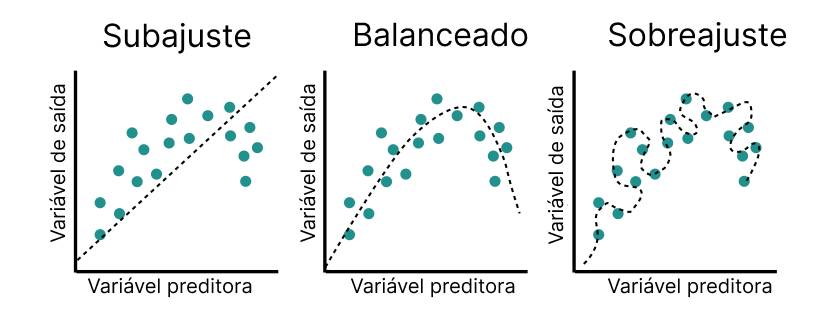
\includegraphics[width=15cm]{figures/fittings.png} % leia abaixo
\legend{Fonte: \citeonline{educative2022overfitting}}
\label{fig:fittings}
\end{figure}